
\title{Thermal building system}
% Use \titlerunning{Short Title} for an abbreviated version of your contribution title if the original one is too long
\author{Roel De Coninck and Lieve Helsen}
\authorrunning{R. De Coninck, L. Helsen}

\maketitle

\abstract{A dynamic thermal system model is developed in Modelica for integrated energy simulation.}

\section{Introduction}

The library is based on Modelica.Thermal.FluidHeatFlow and not on Modelica.Fluid or Modelica.Media.  This makes the library easier to compile by a variety of tools that might not (yet) fully support the  Modelica.Fluid and Modelica.Media libraries.

\section{Hydraulic components}

\subsection{Basic components for Joe the plumber}

\begin{enumerate}
	\item pipe
	\item pump
	\item ambient
	\item three-way valve
	\item pressure grounding
\end{enumerate}

\subsection{Thermal energy storage tank}

\subsubsection{Buffer tank}

\emph{IDEAS.Thermal.Components.Storage.StorageTank}

Buffer tank (no internal heat exhcangers) composed of an array of interconnected pipes with ambient heat losses (= layers).  The number of layers $nbrNodes$ is a parameter and an array of $nbrNodes + 1$ \emph{FlowPort} connectors is available to connect to each intersection between the layers. 

To be completed with schematic, explanation of the heat transfer equations, ambient heat losses, the mixing in case of temperature inversion (buoancy model) and other details.

\subsubsection{Tank with internal heat exchanger}

\emph{IDEAS.Thermal.Components.Storage.StorageTank_OneIntHX}

\vspace{6mm}

This tank is similar to \emph{IDEAS.Thermal.Components.Storage.StorageTank} except that an internal heat exchanger is added.  The heat exchanger can be positioned in any continuous section of layers, it is modelled with one heat exhanger node per tank layer. 

\begin{figure}%
\begin{left}
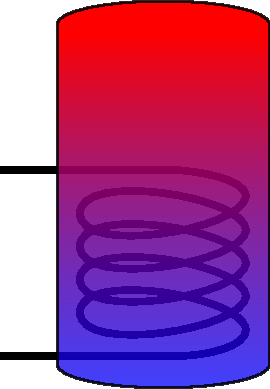
\includegraphics[width=3cm]{Thermal/images/HydraulicScheme.pdf}% of \columnwidth
\caption{Tank with internal heat exchanger}%
\label{tankinternal}%	
\end{left}
\end{figure}

Add heat transfer coefficients and other details.

\subsection{Heat production}

\subsubsection{Partial heater}

\emph{IDEAS.Thermal.Components.Production.Auxiliaries.PartialDynamicHeaterWithLosses}

\vspace{6mm}

All hydraulic heater models extend from this partial heater model.  
tbc

\subsubsection{Boiler}

\subsubsection{Heat pumps}

\begin{enumerate}
	\item modulating air-source hp
	\item ground-source hp
\end{enumerate}

\subsection{Heat emission}

\subsubsection{Partial heat emission model}

\emph{IDEAS.Thermal.Components.Emission.Auxiliaries.Partial_Emission}
\vspace{6mm}

\subsubsection{Radiator}

\subsubsection{Embedded pipe for thermally activated building systems (TABS)}

From ~\cite{Koschenz2000}

\section{Heating systems}

\subsection{Ideal heating}

\subsection{Hydraulic heating}

Main hydraulic scheme with replaceable models for heat production, heat emission, solar thermal system and control.

\subsection{Solar thermal system}

\subsection{Domestic hot water production}

\section{Vertical ground heat exchanger}

\subsection{Model Harm Leenders}

\subsection{Model Dieter Patteeuw}

\section{Control}


%\bibliography{Thermal/MyBibTexLibrary}









